% Digital Logic Report Template
% Created: 2020-01-10, John Miller

%==========================================================
%=========== Document Setup  ==============================

% Formatting defined by class file
\documentclass[11pt]{article}

% ---- Document formatting ----
\usepackage[margin=1in]{geometry}	% Narrower margins
\usepackage{booktabs}				% Nice formatting of tables
\usepackage{graphicx}				% Ability to include graphics

%\setlength\parindent{0pt}	% Do not indent first line of paragraphs 
\usepackage[parfill]{parskip}		% Line space b/w paragraphs
%	parfill option prevents last line of pgrph from being fully justified

% Parskip package adds too much space around titles, fix with this
\RequirePackage{titlesec}
\titlespacing\section{0pt}{8pt plus 4pt minus 2pt}{3pt plus 2pt minus 2pt}
\titlespacing\subsection{0pt}{4pt plus 4pt minus 2pt}{-2pt plus 2pt minus 2pt}
\titlespacing\subsubsection{0pt}{2pt plus 4pt minus 2pt}{-6pt plus 2pt minus 2pt}

% ---- Hyperlinks ----
\usepackage[colorlinks=true,urlcolor=blue]{hyperref}	% For URL's. Automatically links internal references.

% ---- Code listings ----
\usepackage{listings} 					% Nice code layout and inclusion
\usepackage[usenames,dvipsnames]{xcolor}	% Colors (needs to be defined before using colors)

% Define custom colors for listings
\definecolor{listinggray}{gray}{0.98}		% Listings background color
\definecolor{rulegray}{gray}{0.7}			% Listings rule/frame color

% Style for Verilog
\lstdefinestyle{Verilog}{
	language=Verilog,					% Verilog
	backgroundcolor=\color{listinggray},	% light gray background
	rulecolor=\color{blue}, 			% blue frame lines
	frame=tb,							% lines above & below
	linewidth=\columnwidth, 			% set line width
	basicstyle=\small\ttfamily,	% basic font style that is used for the code	
	breaklines=true, 					% allow breaking across columns/pages
	tabsize=3,							% set tab size
	commentstyle=\color{gray},	% comments in italic 
	stringstyle=\upshape,				% strings are printed in normal font
	showspaces=false,					% don't underscore spaces
}

% How to use: \Verilog[listing_options]{file}
\newcommand{\Verilog}[2][]{%
	\lstinputlisting[style=Verilog,#1]{#2}
}




%======================================================
%=========== Body  ====================================
\begin{document}

\title{ELC 2137 Lab 3: Adders}
\author{Trevor Jackson, Carlos Hernandez, and Makenna Meyers}

\maketitle


\section*{Summary}

This lab introduced a family of logic chips that can be used to design logic circuits. Using prior knowledge of AND and XOR gates, Half Adder, Full Adder, and 2-Bit Adder circuits were constructed with these chips and tested for functionality. The schematics and wiring diagrams for the Half Adder and Full Adder circuits can be found in Figure \ref{fig:Circuit_Demonstration}. The Full Adder is merely two Half Adders combined, and the 2-Bit Adder is two Full Adders combined. Figure \ref{fig:Half_Adder} shows the Half Adder circuit built in lab, Figure \ref{fig:Full_Adder} shows the Full Adder circuit, and Figure \ref{fig:2_Bit_Adder} shows the 2-Bit Adder circuit.

\section*{Q\&A}

\begin{enumerate}
	\item Which gates could we use for combining the carry bits?
	
An AND gate or an XOR gate could be used for combining the carry bits.
	
	\item Which one should we use and why?

An XOR gate should be used to combine the carry bits because it will produce a high output when either input is high. As proved in Table \ref{tbl:truth_table}, the carry outputs of the first and second stage Half Adders cannot both be high at the same time, so an AND gate, which produces a high output when both inputs are high, would be ineffective.
   
\end{enumerate}

\section*{Results}

\begin{table}[ht]\centering
	\caption{Truth Table Proving Effectiveness of XOR Gate}
	\label{tbl:truth_table}
	\begin{tabular}{ccc|ccc}
    	\toprule
    	Cin & A & B & A AND B & A XOR B & Cin AND (A XOR B) \\
    	\midrule
    	0 & 0 & 0 & 0 & 0 & 0 \\
    	0 & 0 & 1 & 0 & 1 & 0 \\
    	0 & 1 & 0 & 0 & 1 & 0 \\
    	0 & 1 & 1 & 1 & 0 & 0 \\
    	1 & 0 & 0 & 0 & 0 & 0 \\
    	1 & 0 & 1 & 0 & 1 & 1 \\
    	1 & 1 & 0 & 0 & 1 & 1 \\
    	1 & 1 & 1 & 1 & 0 & 0 \\
    	\bottomrule
    \end{tabular} 
\end{table}

A AND B and Cin AND (A XOR B) are never high at the same time (i.e. they never have 1s at the same time), so an XOR gate can be used to combine them instead of an OR gate. OR gates produce high outputs when either input is high and when both inputs are high, but XOR gates only produce high outputs when either input is high. Because neither input is high at the same time in the Full Adder circuit, an OR gate is not necessary, and an XOR gate can be used.

\begin{figure}\centering
	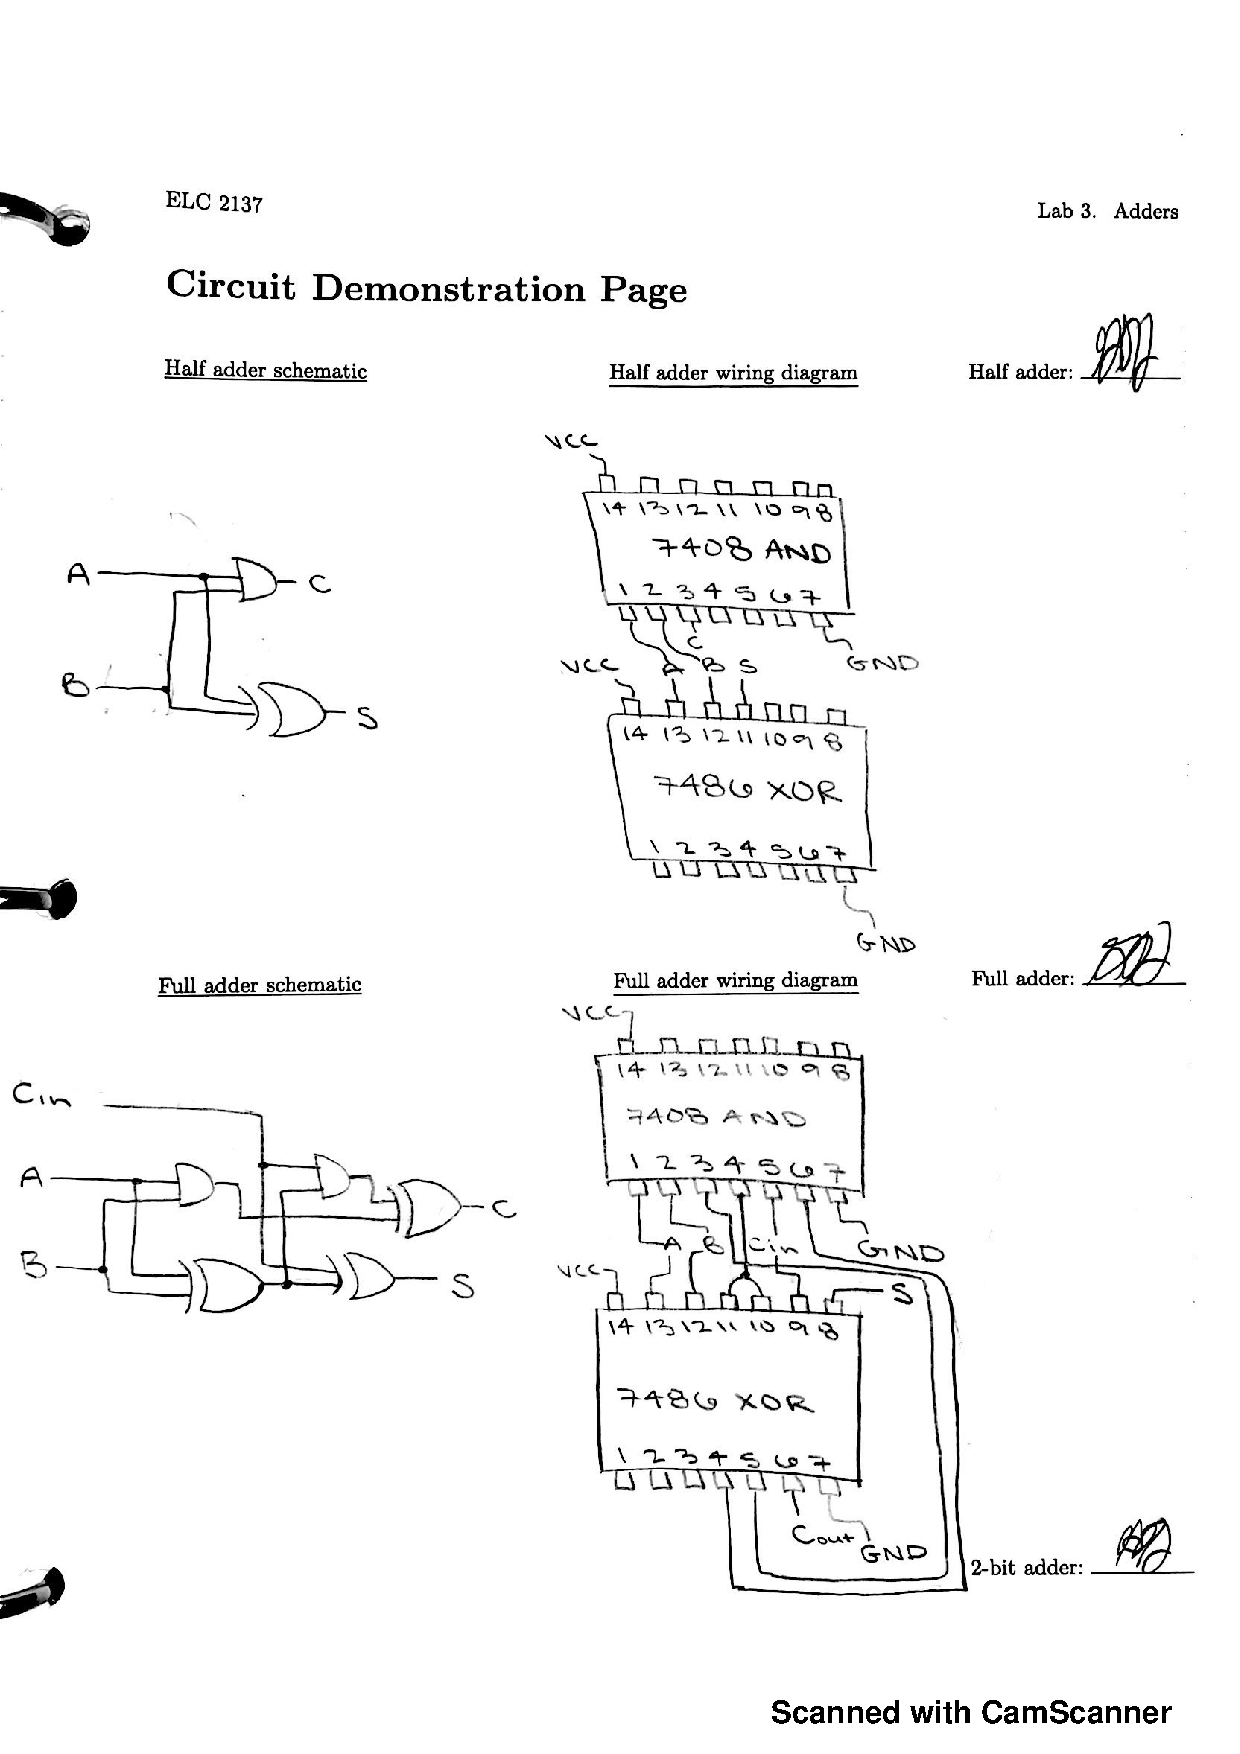
\includegraphics[width=0.8\textwidth,trim=0cm 0cm 0cm 0cm,clip]{Lab3_Circuit_Demonstration_Page} 
	\caption{In-Class Circuit Demonstration}
	\label{fig:Circuit_Demonstration}
\end{figure}	

\begin{figure}\centering
	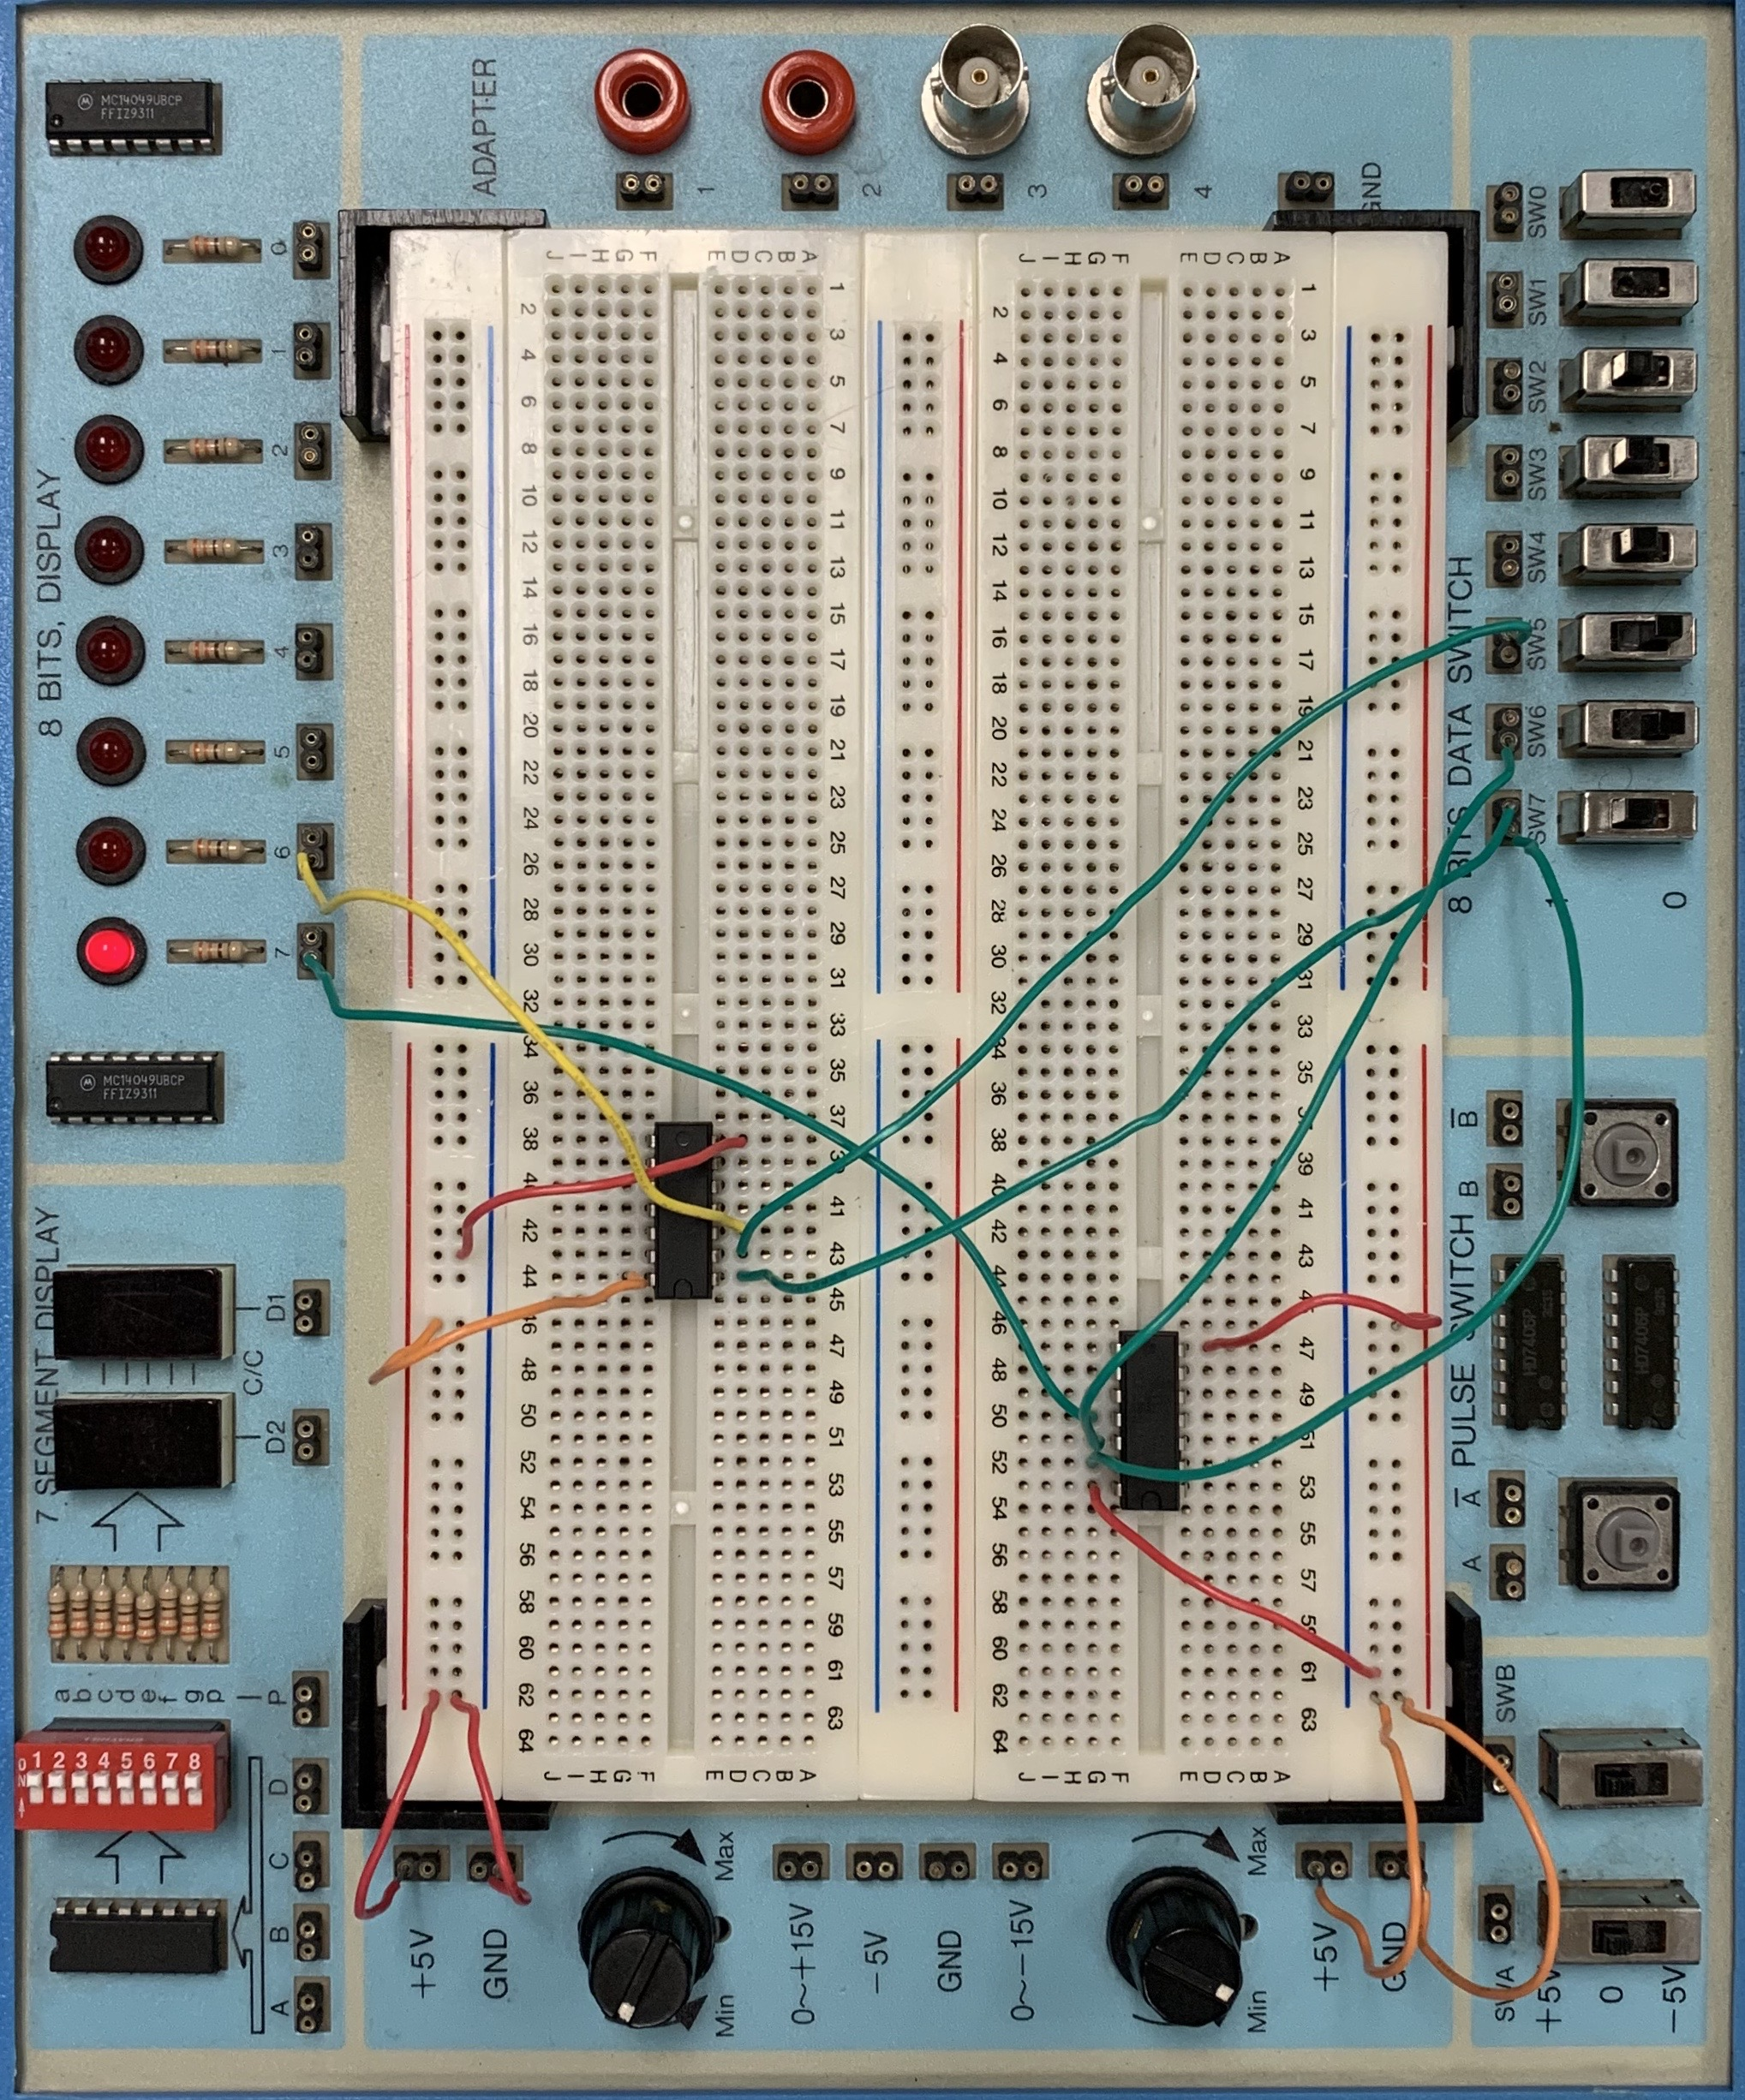
\includegraphics[width=0.8\textwidth,trim=0cm 0cm 0cm 0cm,clip]{Half_Adder}
	\caption{Half Adder Circuit}
	\label{fig:Half_Adder}	
\end{figure}

\begin{figure}\centering
	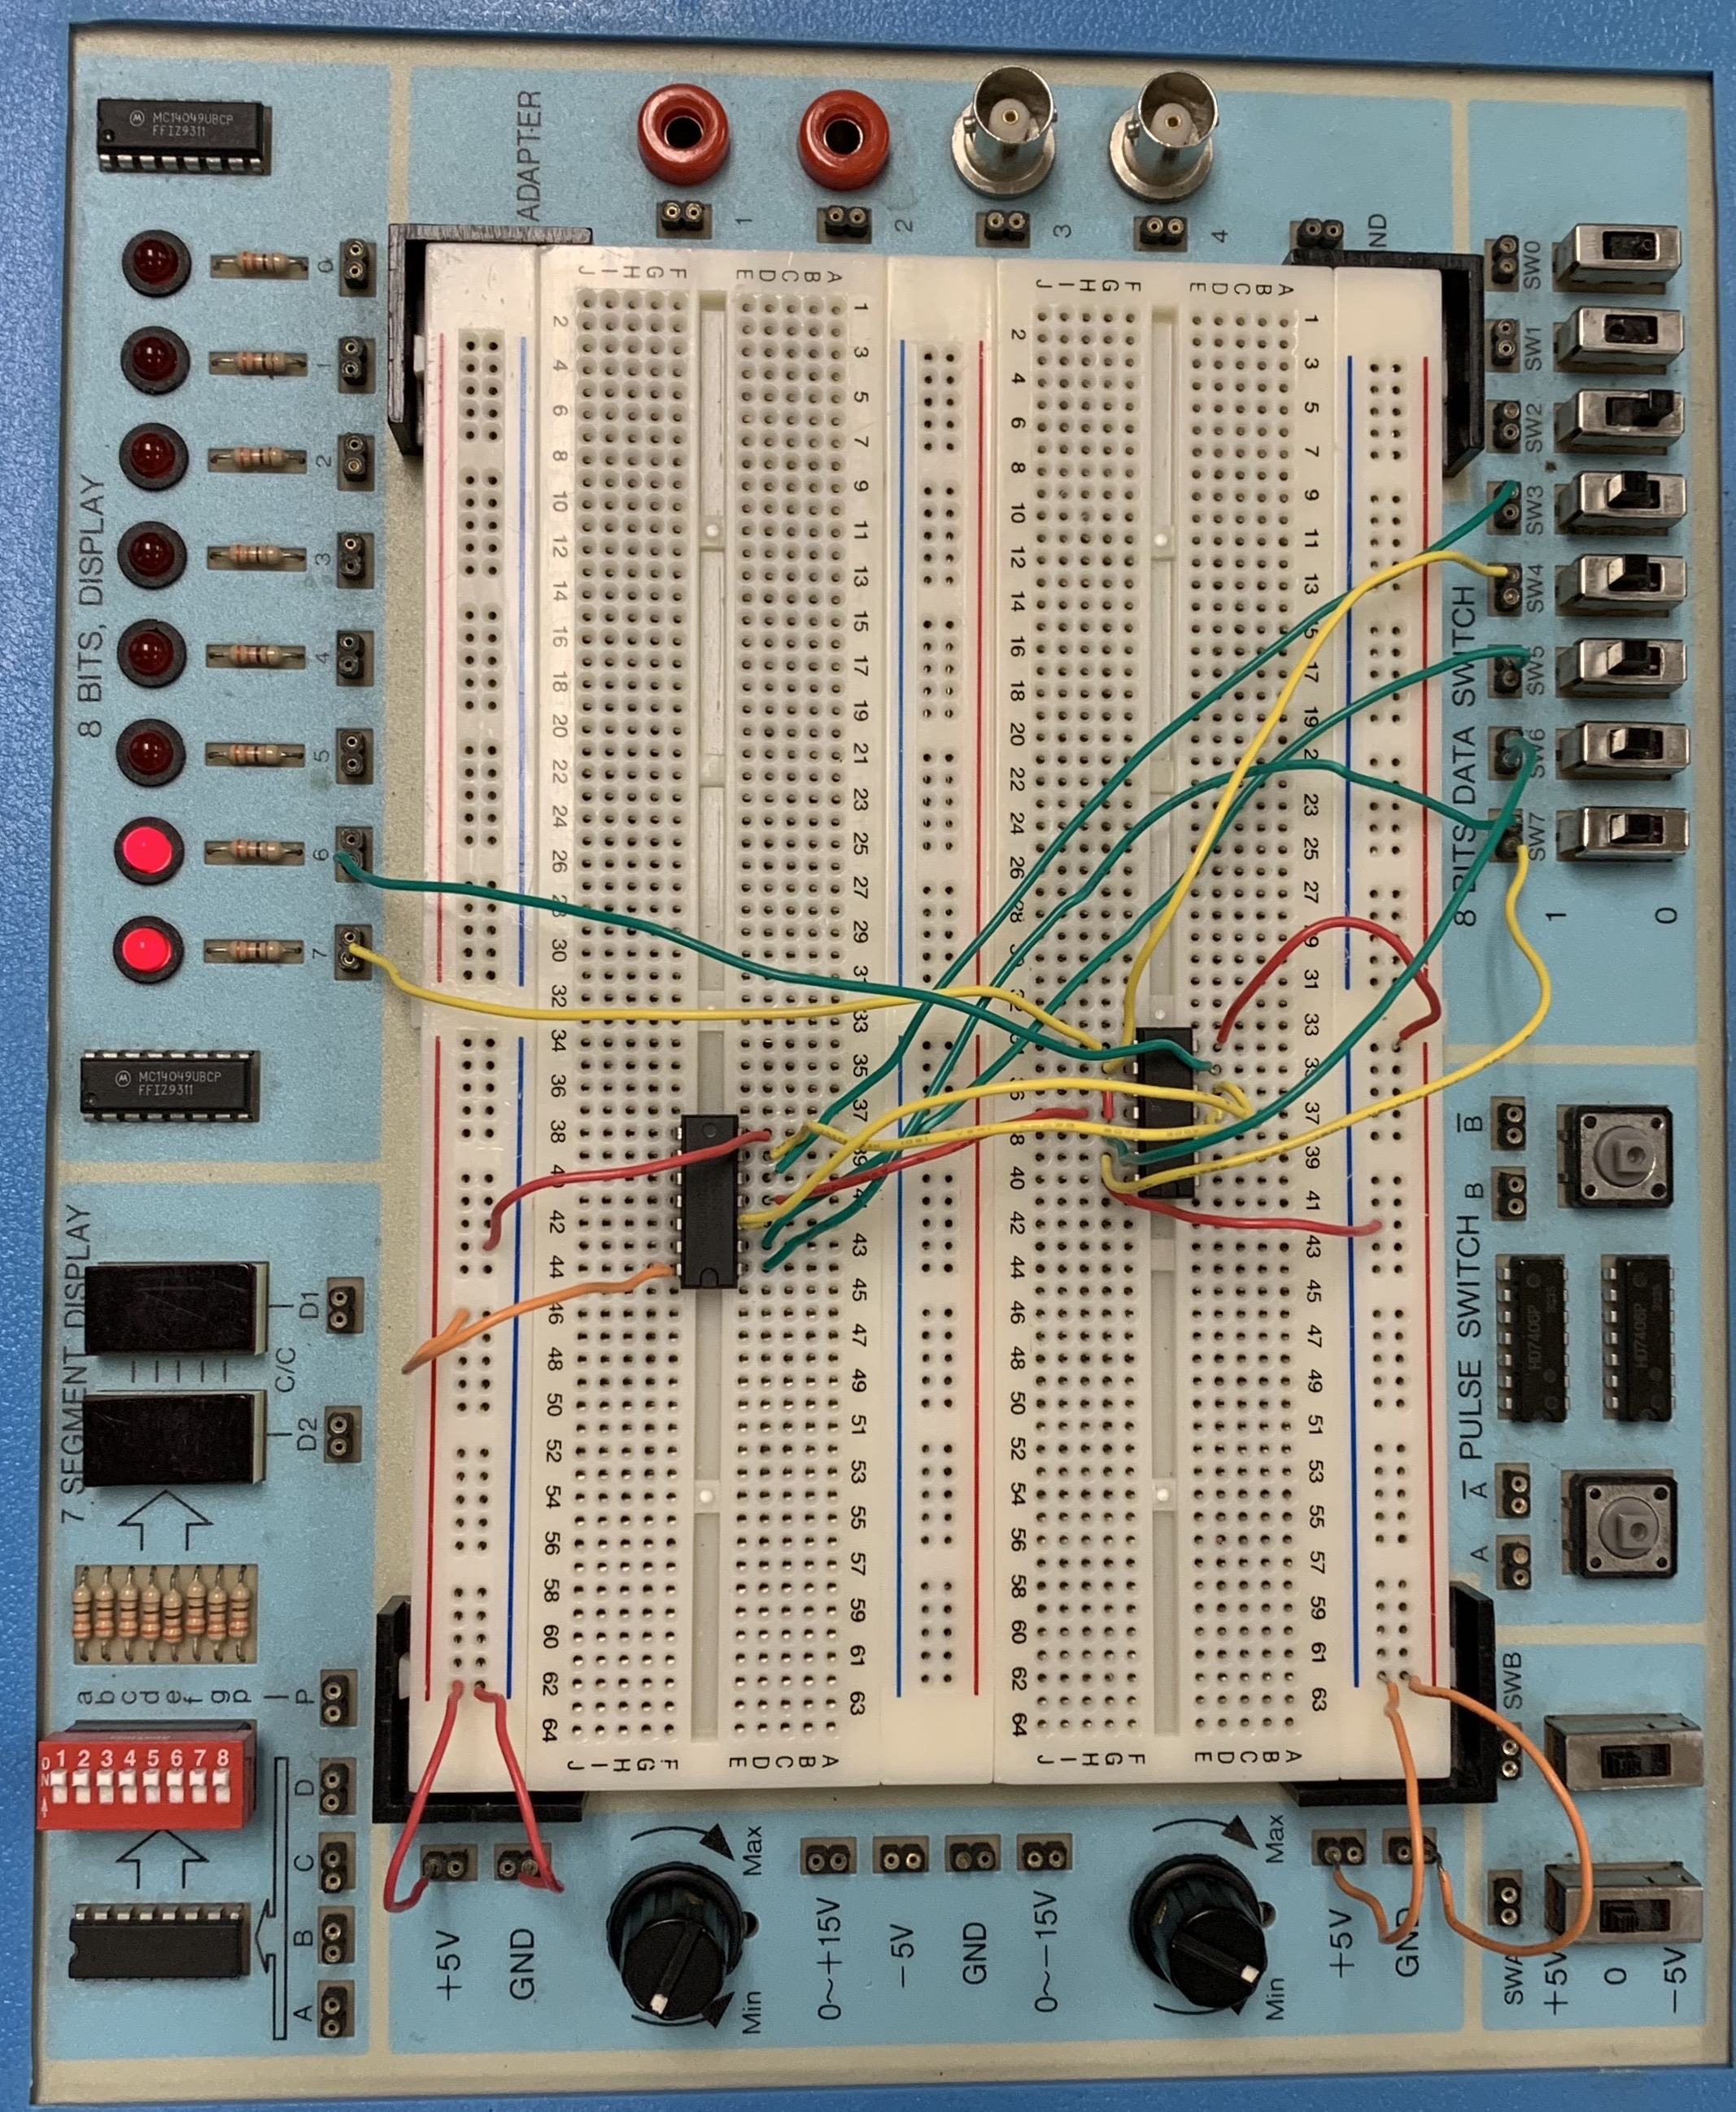
\includegraphics[width=0.8\textwidth,trim=0cm 0cm 0cm 0cm,clip]{Full_Adder}
	\caption{Full Adder Circuit}
	\label{fig:Full_Adder}	
\end{figure}

\begin{figure}\centering
	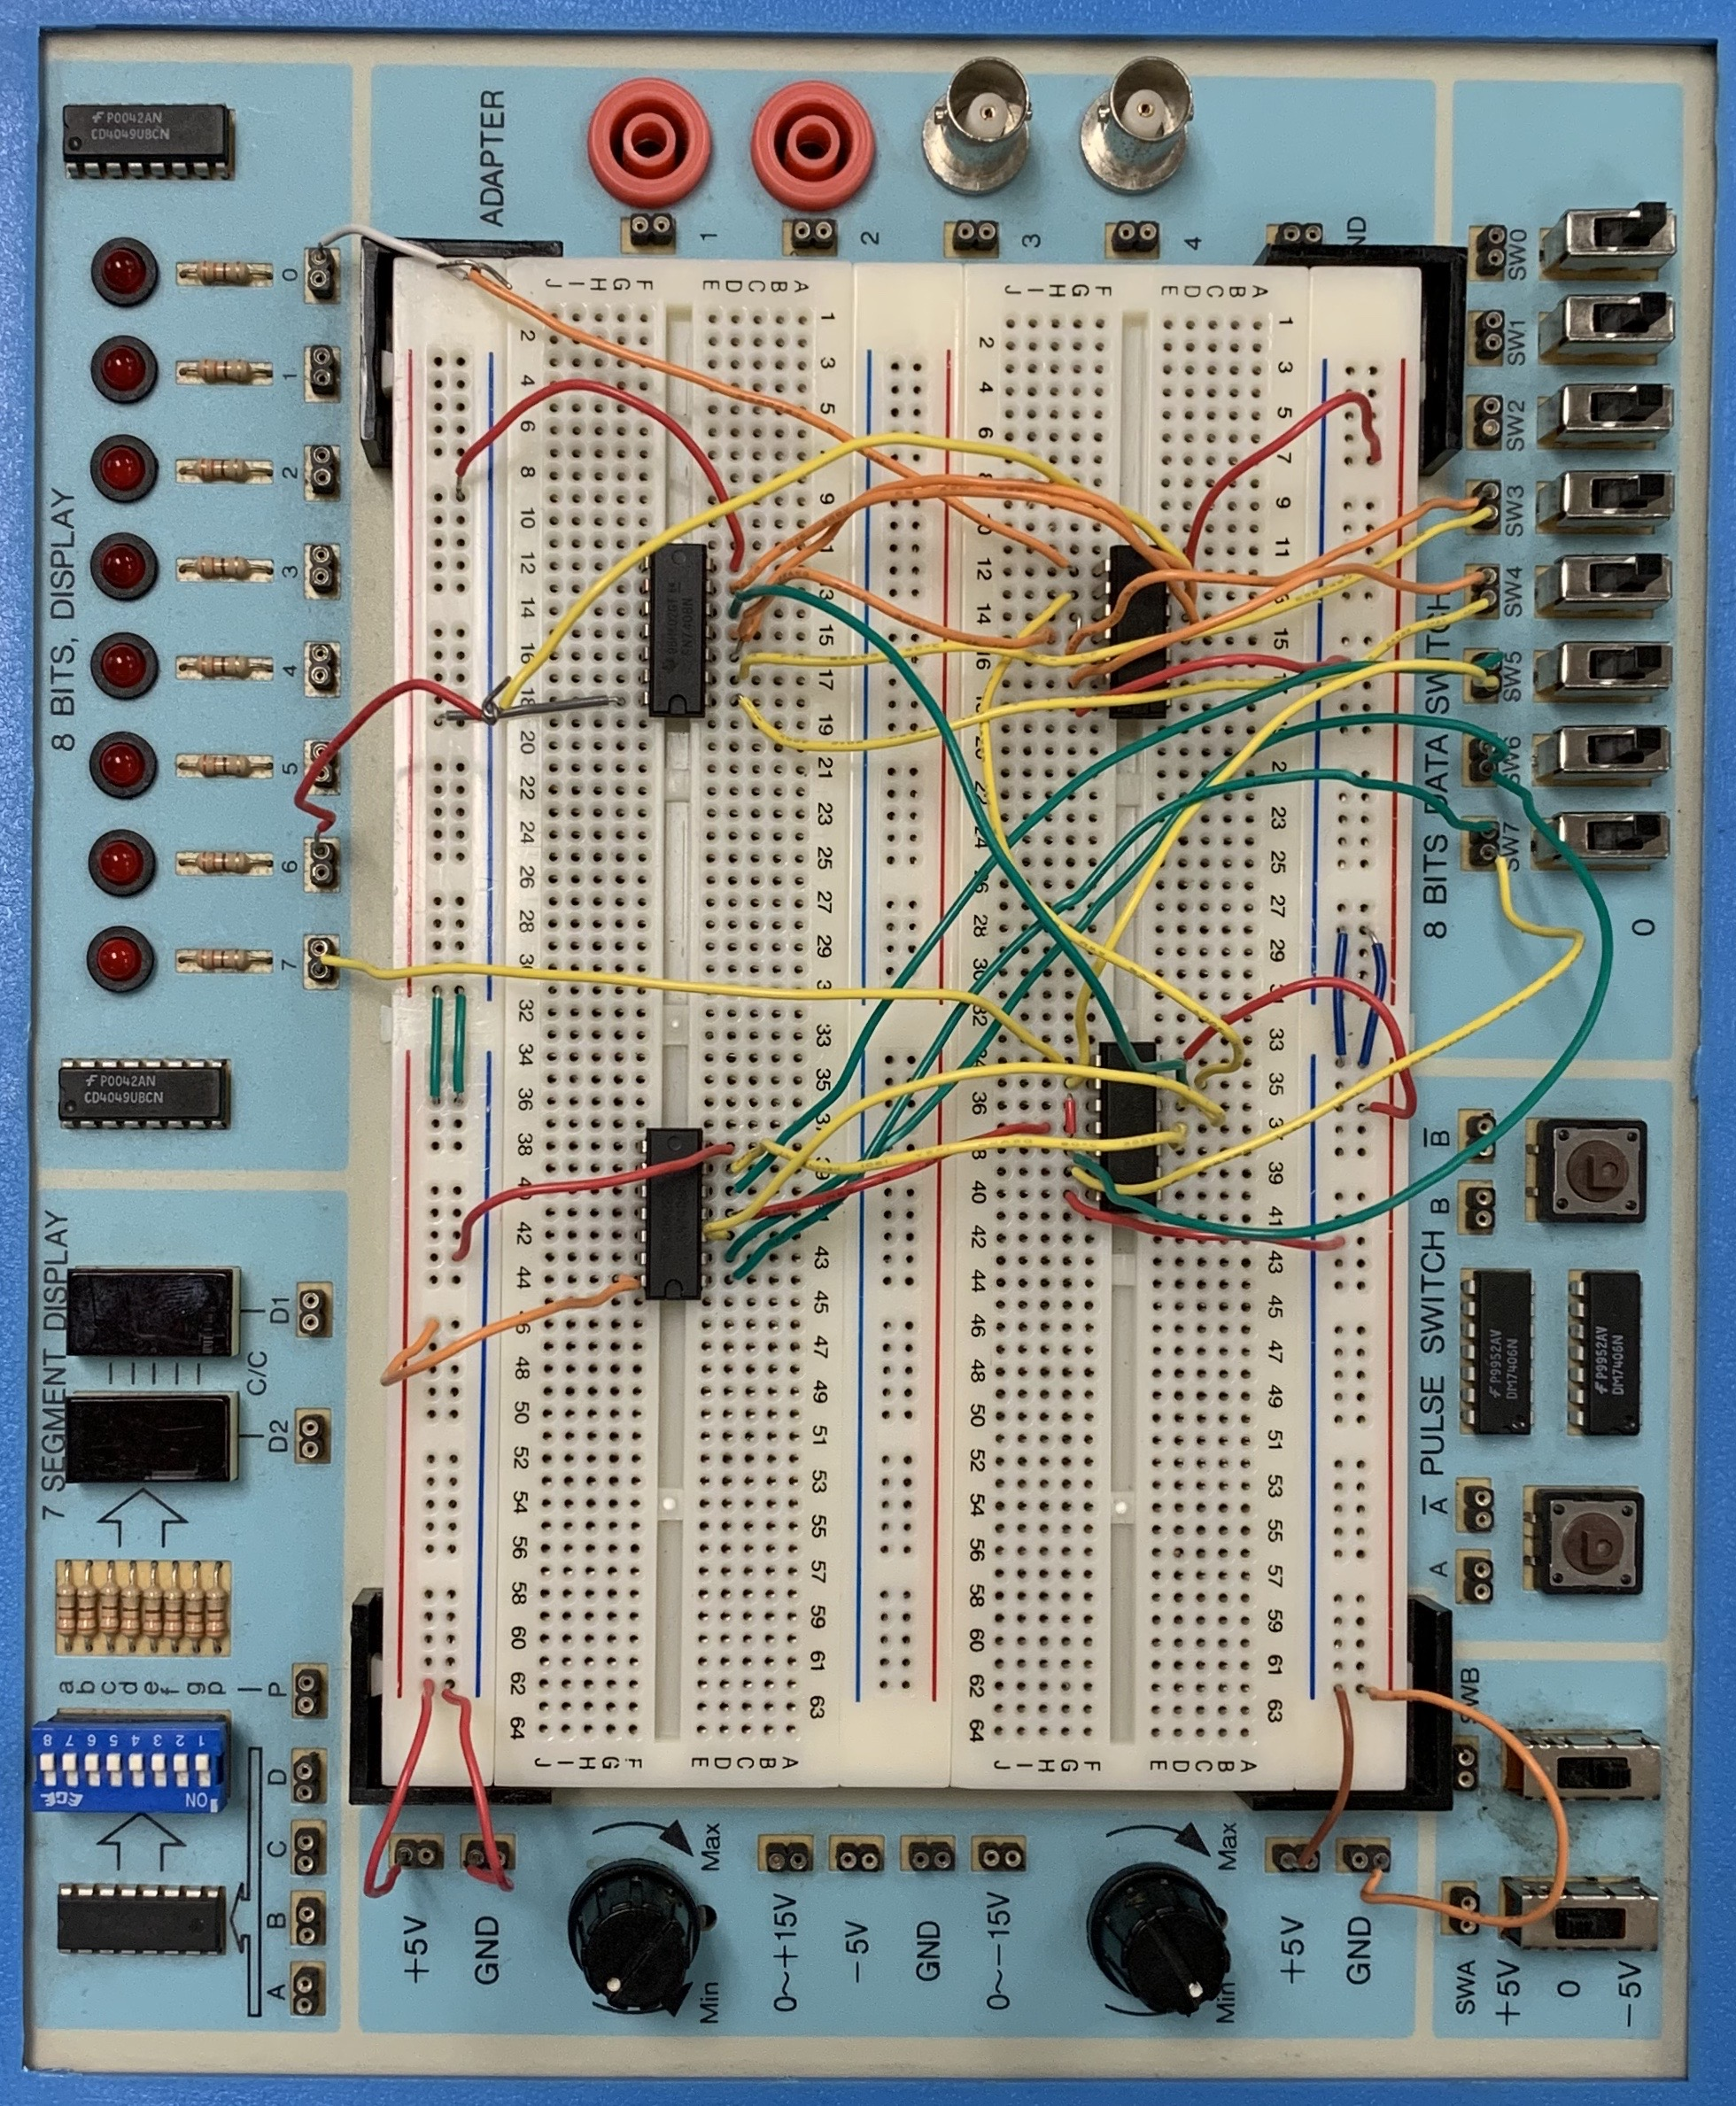
\includegraphics[width=0.8\textwidth,trim=0cm 0cm 0cm 0cm,clip]{2_Bit_Adder}
	\caption{2-Bit Adder Circuit}
	\label{fig:2_Bit_Adder}	
\end{figure}

\clearpage

The connections in some of the switches on the blue box were problematic, so we had to incorporate additional wires and switches to let the Half Adder and Full Adder circuits function properly. A different blue box, with functional switches and connections, was used to build the 2-Bit Adder circuit.

\end{document}
